% vim:noet:sts=2:ts=2:sw=2:smarttab:tw=120

\begin{titlepage}
	\begin{german}
		\makecoverpage{%
			Lehrstuhl für Informatik 4 $\cdot$ Verteilte Systeme und Betriebssysteme
		}{%
			\thesisauthor%
		}{%
			\thesistitle%
		}{%
			Masterarbeit im Fach \thesissubject\\[3ex]%
			\displaydate{thesisenddate}%
		}{%
			\begin{english}
				Please cite as:\\%
				\nohyphens{\thesisauthor{}, \enquote{\thesistitle}, Master's Thesis, University of Erlangen, Dept.\ of Computer
				Science, \citationdate\displaydate{thesisenddate}.}
			\end{english}
		}{%
			\begin{german}
				Friedrich-Alexander-Universität Erlangen-Nürnberg\\%
				Department Informatik\\%
				Verteilte Systeme und Betriebssysteme\\%
				\vspace{.5em}%
				Martensstr. 1 $\cdot$ 91058 Erlangen $\cdot$ Germany%
			\end{german}
		}{%
			\href{https://www4.cs.fau.de/}{www4.cs.fau.de}%
		}{%
			
\includegraphics[width=76.4mm]{images/i4/Logo_Tech-Fak_DinA4_4C}%
		}{%
			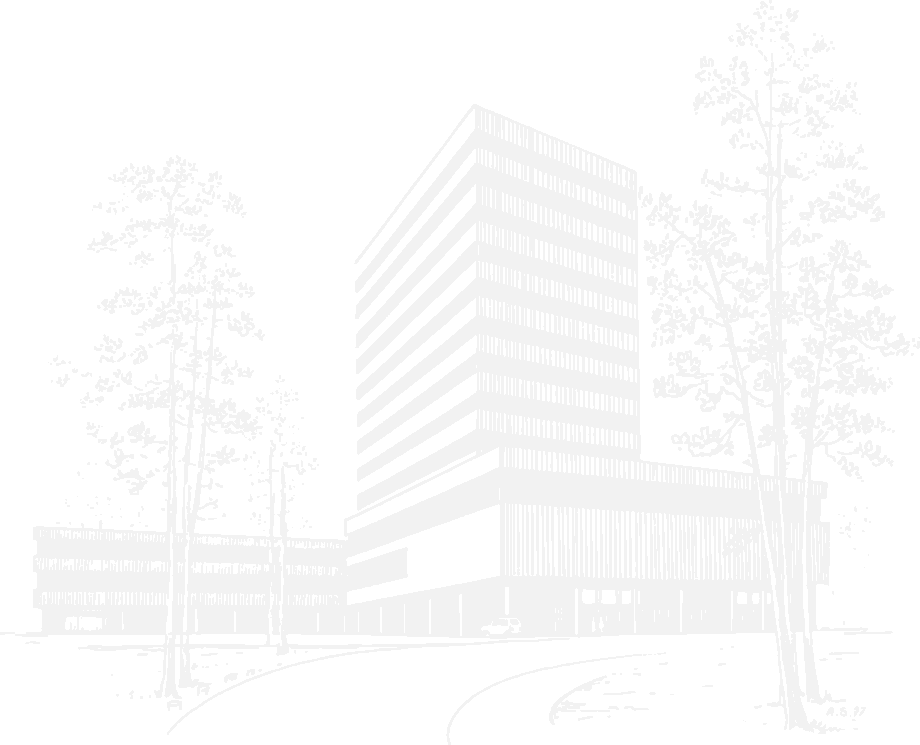
\includegraphics{images/i4/watermark-inf.pdf}%
		}

		\clearpage
		\thispagestyle{empty}
		\begin{flushright}
			\rmfamily
			{\LARGE\thesistitle{}}\\
			\begin{small}
				Masterarbeit im Fach \thesissubject{}\\
				\vspace*{1cm}
				von \textbf{\thesisauthor{}}\\
				geboren am \displaydate{thesisbirthdate} in \thesisbirthlocation{}\\
				\vspace{\fill}
				\textbf{Lehrstuhl für Informatik 4}\\
				Friedrich-Alexander Universität Erlangen-Nürnberg\\
				\vspace*{1cm}
				\textbf{Betreut durch}\\
				\thesisadvisors{}\\
				\vspace*{1cm}
				\begin{tabular}{rr}
					\textbf{Beginn:} & \displaydate{thesisstartdate} \\
					\textbf{Abgabe:} & \displaydate{thesisenddate}
				\end{tabular}
			\end{small}
		\end{flushright}
	\end{german}
\end{titlepage}
